\documentclass[11pt]{article}
\usepackage{amsmath, amsfonts, amsthm, amssymb}  % Some math symbols
\usepackage{lmodern}  % A modern version of LaTeX's famous default font. 
\usepackage{microtype}
\usepackage{fullpage}

\usepackage[x11names, rgb]{xcolor}
\usepackage{graphicx}
\usepackage{tikz}
\usetikzlibrary{decorations,arrows,shapes}

\usepackage{etoolbox}
\usepackage{enumerate}
\usepackage{listings}

\setlength{\parindent}{0pt}
\setlength{\parskip}{5pt plus 1pt}

\newcommand{\nopagenumbers}{
    \pagestyle{empty}
}

\def\indented#1{\list{}{}\item[]}
\let\indented=\endlist

\providetoggle{questionnumbers}
\settoggle{questionnumbers}{true}
\newcommand{\noquestionnumbers}{
    \settoggle{questionnumbers}{false}
}

\newcounter{questionCounter}
\newenvironment{question}[2][\arabic{questionCounter}]{%
    \addtocounter{questionCounter}{1}%
    \setcounter{partCounter}{0}%
    \vspace{.25in} \hrule \vspace{0.4em}%
        \noindent{\bf \iftoggle{questionnumbers}{#1: }{}#2}%
    \vspace{0.8em} \hrule \vspace{.10in}%
}{$ $\newpage}

\newcounter{partCounter}[questionCounter]
\renewenvironment{part}[1][\alph{partCounter}]{%
    \addtocounter{partCounter}{1}%
    \vspace{.10in}%
    \begin{indented}%
       {\bf (#1)} %
}{\end{indented}}

\def\show#1{\ifdefempty{#1}{}{#1\\}}




%%%%%%%%%%%%%%%%% Identifying Information %%%%%%%%%%%%%%%%%
%% For 301, we'd rather you DIDN'T tell us who you are   %%
%% in your homework so that we're not biased when we     %%
%% grade. So, even if you fill this information in, it   %%
%% will not show up in the document unless you uncomment %%
%% \show\myname and \show\myemail below                  %%
%%%%%%%%%%%%%%%%%%%%%%%%%%%%%%%%%%%%%%%%%%%%%%%%%%%%%%%%%%%
\newcommand{\myhwname}{Homework 1}
\newcommand{\myname}{John Ezra See}
\newcommand{\myemail}{jsee4@uic.edu}
%%%%%%%%%%%%%%%%%%%%%%%%%%%%%%%%%%%%%%%%%%%%%%%%%%%%%%%%%%%
\newcommand{\header}{%
\begin{center}
    {\Large \show\myhwname}
    % \show\myname
    % \show\myemail
    \today
\end{center}}
%%%%%%%%%%%%%%%%%%% Document Options %%%%%%%%%%%%%%%%%%%%%%
% \noquestionnumbers
\nopagenumbers
%%%%%%%%%%%%%%%%%%%%%%%%%%%%%%%%%%%%%%%%%%%%%%%%%%%%%%%%%%%

\begin{document}
\header

\begin{question}{Deterministic Construction}
    \begin{part} 
        \begin{center}
            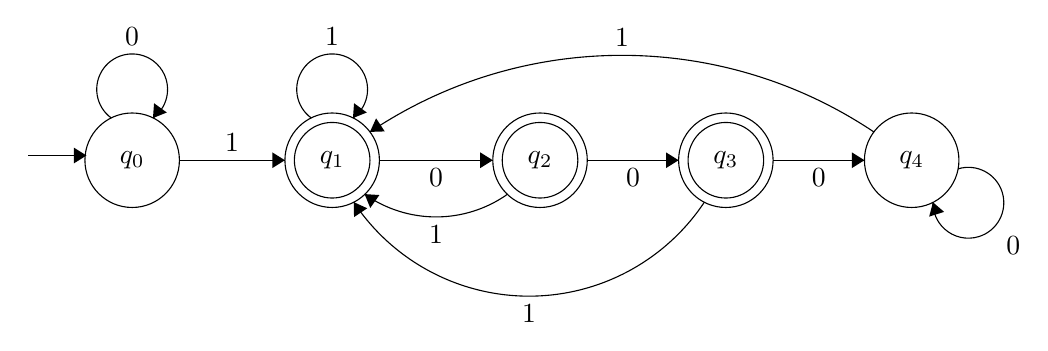
\begin{tikzpicture}[scale=0.2]
            \tikzstyle{every node}+=[inner sep=0pt]
            \draw [black] (7.9,-14.2) circle (3);
            \draw (7.9,-14.2) node {$q_0$};
            \draw [black] (20.6,-14.2) circle (3);
            \draw (20.6,-14.2) node {$q_1$};
            \draw [black] (20.6,-14.2) circle (2.4);
            \draw [black] (33.8,-14.2) circle (3);
            \draw (33.8,-14.2) node {$q_2$};
            \draw [black] (33.8,-14.2) circle (2.4);
            \draw [black] (45.6,-14.2) circle (3);
            \draw (45.6,-14.2) node {$q_3$};
            \draw [black] (45.6,-14.2) circle (2.4);
            \draw [black] (57.4,-14.2) circle (3);
            \draw (57.4,-14.2) node {$q_4$};
            \draw [black] (10.9,-14.2) -- (17.6,-14.2);
            \fill [black] (17.6,-14.2) -- (16.8,-13.7) -- (16.8,-14.7);
            \draw [black] (1.3,-13.9) -- (5,-13.9);
            \fill [black] (5,-13.9) -- (4.2,-13.4) -- (4.2,-14.4);
            \draw (14.25,-13.7) node [above] {$1$};
            \draw [black] (36.8,-14.2) -- (42.6,-14.2);
            \fill [black] (42.6,-14.2) -- (41.8,-13.7) -- (41.8,-14.7);
            \draw (39.7,-14.7) node [below] {$0$};
            \draw [black] (48.6,-14.2) -- (54.4,-14.2);
            \fill [black] (54.4,-14.2) -- (53.6,-13.7) -- (53.6,-14.7);
            \draw (51.5,-14.7) node [below] {$0$};
            \draw [black] (6.577,-11.52) arc (234:-54:2.25);
            \draw (7.9,-6.95) node [above] {$0$};
            \fill [black] (9.22,-11.52) -- (10.1,-11.17) -- (9.29,-10.58);
            \draw [black] (19.277,-11.52) arc (234:-54:2.25);
            \draw (20.6,-6.95) node [above] {$1$};
            \fill [black] (21.92,-11.52) -- (22.8,-11.17) -- (21.99,-10.58);
            \draw [black] (23.6,-14.2) -- (30.8,-14.2);
            \fill [black] (30.8,-14.2) -- (30,-13.7) -- (30,-14.7);
            \draw (27.2,-14.7) node [below] {$0$};
            \draw [black] (31.739,-16.355) arc (-54.67556:-125.32444:7.85);
            \fill [black] (22.66,-16.35) -- (23.02,-17.23) -- (23.6,-16.41);
            \draw (27.2,-18.3) node [below] {$1$};
            \draw [black] (44.233,-16.863) arc (-33.606:-146.394:13.367);
            \fill [black] (21.97,-16.86) -- (21.99,-17.81) -- (22.83,-17.25);
            \draw (33.1,-23.33) node [below] {$1$};
            \draw [black] (23.001,-12.403) arc (123.82847:56.17153:28.739);
            \fill [black] (23,-12.4) -- (23.94,-12.37) -- (23.39,-11.54);
            \draw (39,-7.04) node [above] {$1$};
            \draw [black] (60.337,-14.75) arc (107.1301:-180.8699:2.25);
            \draw (63.38,-19.65) node [right] {$0$};
            \fill [black] (58.75,-16.87) -- (58.51,-17.78) -- (59.46,-17.48);
            \end{tikzpicture}
            \end{center}
    \end{part}

    \begin{part}

        $Q = \{q_0, q_1, q_2, q_3, q_4\}$ \\
        $\sum = \{0, 1\}$ \\
        $q_0 = q_0$ \\ 
        $F = \{q_1, q_2, q_3\}$ \\
        $\delta = $ See Table 1

        \begin{table}[ht]
            \centering
            \begin{tabular}{|c|c|c|}
              \hline
                & 0 & 1 \\
              \hline
              $q_0$ & $q_0$ & $q_1$ \\
              $q_1$ & $q_2$ & $q_1$ \\
              $q_2$ & $q_3$ & $q_1$ \\
              $q_3$ & $q_4$ & $q_1$ \\
              $q_4$ & $q_4$ & $q_1$ \\
              \hline
            \end{tabular}
            \caption{Transition Function}
            \label{tab:four_by_two_labels}
          \end{table}

    \end{part}
\end{question}

\begin{question}{Nondeterministic Construction}
    
\begin{center}
    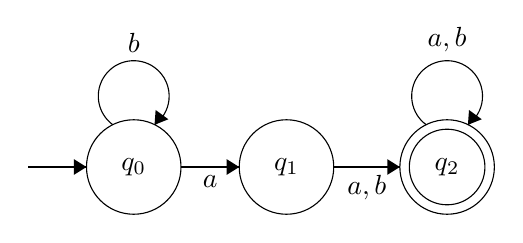
\begin{tikzpicture}[scale=0.2]
    \tikzstyle{every node}+=[inner sep=0pt]
    \draw [black] (8,-13.9) circle (3);
    \draw (8,-13.9) node {$q_0$};
    \draw [black] (17.7,-13.9) circle (3);
    \draw (17.7,-13.9) node {$q_1$};
    \draw [black] (27.9,-13.9) circle (3);
    \draw (27.9,-13.9) node {$q_2$};
    \draw [black] (27.9,-13.9) circle (2.4);
    \draw [black] (1.3,-13.9) -- (5,-13.9);
    \fill [black] (5,-13.9) -- (4.2,-13.4) -- (4.2,-14.4);
    \draw [black] (20.7,-13.9) -- (24.9,-13.9);
    \fill [black] (24.9,-13.9) -- (24.1,-13.4) -- (24.1,-14.4);
    \draw (22.8,-14.4) node [below] {$a,b$};
    \draw [black] (11,-13.9) -- (14.7,-13.9);
    \fill [black] (14.7,-13.9) -- (13.9,-13.4) -- (13.9,-14.4);
    \draw (12.85,-14.4) node [below] {$a$};
    \draw [black] (6.677,-11.22) arc (234:-54:2.25);
    \draw (8,-6.65) node [above] {$b$};
    \fill [black] (9.32,-11.22) -- (10.2,-10.87) -- (9.39,-10.28);
    \draw [black] (26.577,-11.22) arc (234:-54:2.25);
    \draw (27.9,-6.65) node [above] {$a,b$};
    \fill [black] (29.22,-11.22) -- (30.1,-10.87) -- (29.29,-10.28);
    \end{tikzpicture}
    \end{center}    
\end{question}

\begin{question}{NFA to DFA Conversion}
    :: Assume that state AB is equivalent to state \{A, B\}
\begin{center}
    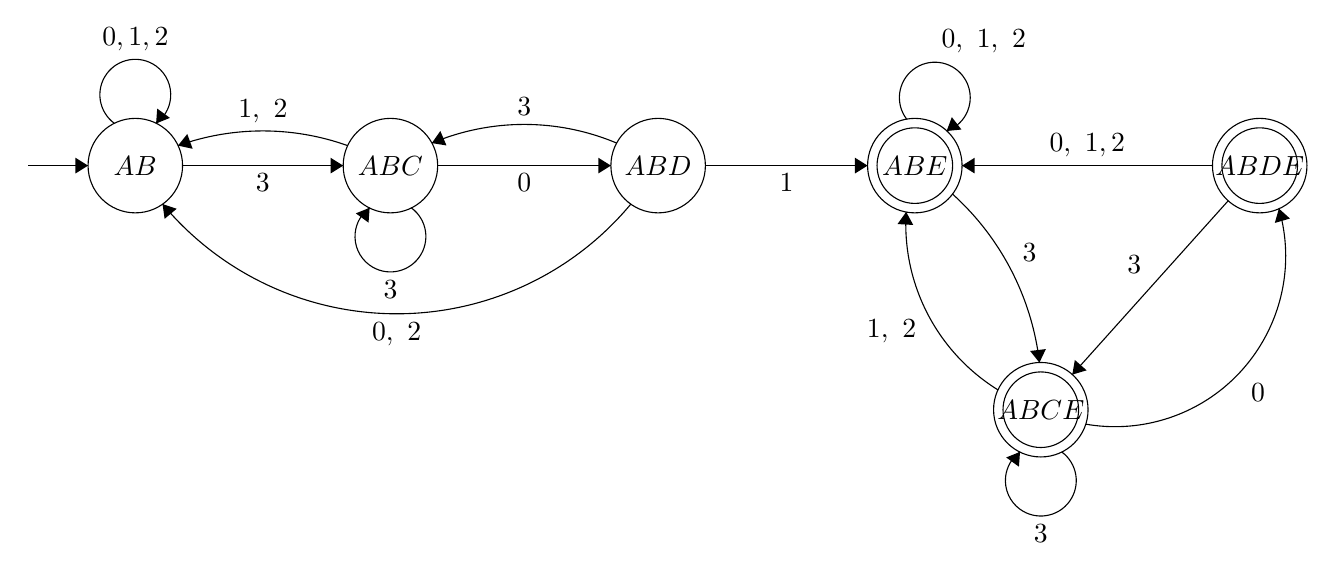
\begin{tikzpicture}[scale=0.2]
    \tikzstyle{every node}+=[inner sep=0pt]
    \draw [black] (5.1,-13.1) circle (3);
    \draw (5.1,-13.1) node {$AB$};
    \draw [black] (21.3,-13.1) circle (3);
    \draw (21.3,-13.1) node {$ABC$};
    \draw [black] (38.3,-13.1) circle (3);
    \draw (38.3,-13.1) node {$ABD$};
    \draw [black] (54.6,-13.1) circle (3);
    \draw (54.6,-13.1) node {$ABE$};
    \draw [black] (54.6,-13.1) circle (2.4);
    \draw [black] (76.5,-13.1) circle (3);
    \draw (76.5,-13.1) node {$ABDE$};
    \draw [black] (76.5,-13.1) circle (2.4);
    \draw [black] (62.6,-28.6) circle (3);
    \draw (62.6,-28.6) node {$ABCE$};
    \draw [black] (62.6,-28.6) circle (2.4);
    \draw [black] (-1.7,-13.1) -- (2.1,-13.1);
    \fill [black] (2.1,-13.1) -- (1.3,-12.6) -- (1.3,-13.6);
    \draw [black] (3.777,-10.42) arc (234:-54:2.25);
    \draw (5.1,-5.85) node [above] {$0,1,2$};
    \fill [black] (6.42,-10.42) -- (7.3,-10.07) -- (6.49,-9.48);
    \draw [black] (8.1,-13.1) -- (18.3,-13.1);
    \fill [black] (18.3,-13.1) -- (17.5,-12.6) -- (17.5,-13.6);
    \draw (13.2,-13.6) node [below] {$3$};
    \draw [black] (7.813,-11.831) arc (109.68995:70.31005:15.987);
    \fill [black] (7.81,-11.83) -- (8.74,-12.03) -- (8.4,-11.09);
    \draw (13.2,-10.4) node [above] {$1,\mbox{ }2$};
    \draw [black] (23.931,-11.669) arc (112.84805:67.15195:15.114);
    \fill [black] (23.93,-11.67) -- (24.86,-11.82) -- (24.47,-10.9);
    \draw (29.8,-9.98) node [above] {$3$};
    \draw [black] (24.3,-13.1) -- (35.3,-13.1);
    \fill [black] (35.3,-13.1) -- (34.5,-12.6) -- (34.5,-13.6);
    \draw (29.8,-13.6) node [below] {$0$};
    \draw [black] (22.623,-15.78) arc (54:-234:2.25);
    \draw (21.3,-20.35) node [below] {$3$};
    \fill [black] (19.98,-15.78) -- (19.1,-16.13) -- (19.91,-16.72);
    \draw [black] (41.3,-13.1) -- (51.6,-13.1);
    \fill [black] (51.6,-13.1) -- (50.8,-12.6) -- (50.8,-13.6);
    \draw (46.45,-13.6) node [below] {$1$};
    \draw [black] (36.566,-15.544) arc (-39.79286:-140.20714:19.348);
    \fill [black] (6.83,-15.54) -- (6.96,-16.48) -- (7.73,-15.84);
    \draw (21.7,-23.01) node [below] {$0,\mbox{ }2$};
    \draw [black] (54.087,-10.156) arc (217.61046:-70.38954:2.25);
    \draw (58.98,-5.97) node [above] {$0,\mbox{ }1,\mbox{ }2$};
    \fill [black] (56.62,-10.9) -- (57.56,-10.81) -- (56.95,-10.02);
    \draw [black] (56.992,-14.905) arc (47.92965:6.6695:17.088);
    \fill [black] (62.51,-25.61) -- (62.92,-24.75) -- (61.92,-24.87);
    \draw (61.41,-18.62) node [right] {$3$};
    \draw [black] (59.884,-27.344) arc (-121.76498:-183.63587:12.371);
    \fill [black] (54.05,-16.04) -- (53.5,-16.81) -- (54.5,-16.87);
    \draw (54.72,-23.64) node [left] {$1,\mbox{ }2$};
    \draw [black] (73.5,-13.1) -- (57.6,-13.1);
    \fill [black] (57.6,-13.1) -- (58.4,-13.6) -- (58.4,-12.6);
    \draw (65.55,-12.6) node [above] {$0,\mbox{ }1,2$};
    \draw [black] (63.923,-31.28) arc (54:-234:2.25);
    \draw (62.6,-35.85) node [below] {$3$};
    \fill [black] (61.28,-31.28) -- (60.4,-31.63) -- (61.21,-32.22);
    \draw [black] (77.72,-15.83) arc (16.14939:-99.91926:10.835);
    \fill [black] (77.72,-15.83) -- (77.46,-16.74) -- (78.42,-16.46);
    \draw (75.92,-27.53) node [right] {$0$};
    \draw [black] (74.5,-15.33) -- (64.6,-26.37);
    \fill [black] (64.6,-26.37) -- (65.51,-26.1) -- (64.76,-25.44);
    \draw (69.01,-19.39) node [left] {$3$};
    \end{tikzpicture}
    \end{center}
    
    
\end{question}

\begin{question}{Closure in Reverse}
    Proof: \\
    Suppose that the language L is regular. We should prove that the reverse is also regular. \\
    We know that if a language is regular, then there is some NFA that decides that language. \\ 
    Since L is regular, there is an NFA that decides L. We can call the NFA of L, $M_L$. \\
    \[
        \therefore \text{ We must show that there is also an NFA that decides the reverse of } L, \text{ which we will call } M_R.
        \]
        

    To construct $M_R$, we will use the 5-tuples of L. \\
    $Q_R$ = $Q$ (i.e we shall use the same states). \\
    $\sum_R = \sum$ (i.e we shall use the same alphabets) \\
    $F_R$ = $q_0$ (i.e the start state of L will be our final state in $M_R$) \\
    $q_R$ = $ q_0 \cup F$  (i.e the set of final states of L will be our start states connected using epsilon.) \\
    The arrow directions should be swapped but everything else remains the same in the transition function.
    \\ \\ For example, take $M_L$ ::
    
    \begin{center}
    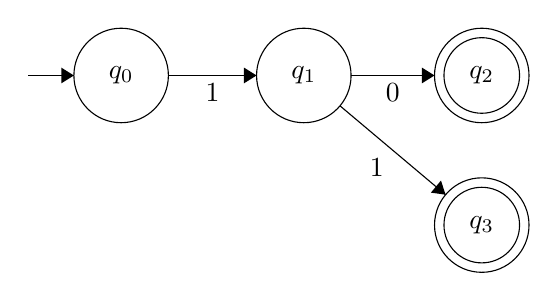
\begin{tikzpicture}[scale=0.2]
    \tikzstyle{every node}+=[inner sep=0pt]
    \draw [black] (20.3,-14.8) circle (3);
    \draw (20.3,-14.8) node {$q_0$};
    \draw [black] (31.9,-14.8) circle (3);
    \draw (31.9,-14.8) node {$q_1$};
    \draw [black] (43.2,-14.8) circle (3);
    \draw (43.2,-14.8) node {$q_2$};
    \draw [black] (43.2,-14.8) circle (2.4);
    \draw [black] (43.2,-24.3) circle (3);
    \draw (43.2,-24.3) node {$q_3$};
    \draw [black] (43.2,-24.3) circle (2.4);
    \draw [black] (14.4,-14.8) -- (17.3,-14.8);
    \fill [black] (17.3,-14.8) -- (16.5,-14.3) -- (16.5,-15.3);
    \draw [black] (23.3,-14.8) -- (28.9,-14.8);
    \fill [black] (28.9,-14.8) -- (28.1,-14.3) -- (28.1,-15.3);
    \draw (26.1,-15.3) node [below] {$1$};
    \draw [black] (34.9,-14.8) -- (40.2,-14.8);
    \fill [black] (40.2,-14.8) -- (39.4,-14.3) -- (39.4,-15.3);
    \draw (37.55,-15.3) node [below] {$0$};
    \draw [black] (34.2,-16.73) -- (40.9,-22.37);
    \fill [black] (40.9,-22.37) -- (40.61,-21.47) -- (39.97,-22.24);
    \draw (36.54,-20.04) node [below] {$1$};
    \end{tikzpicture}
    \end{center}
    
    As a result, $M_R$ :: 

    \begin{center}
    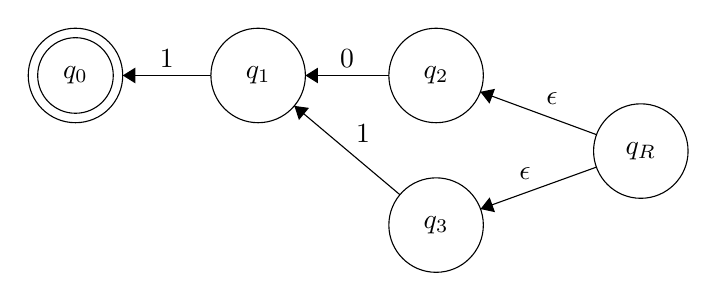
\begin{tikzpicture}[scale=0.2]
    \tikzstyle{every node}+=[inner sep=0pt]
    \draw [black] (20.3,-14.8) circle (3);
    \draw (20.3,-14.8) node {$q_0$};
    \draw [black] (20.3,-14.8) circle (2.4);
    \draw [black] (31.9,-14.8) circle (3);
    \draw (31.9,-14.8) node {$q_1$};
    \draw [black] (43.2,-14.8) circle (3);
    \draw (43.2,-14.8) node {$q_2$};
    \draw [black] (43.2,-24.3) circle (3);
    \draw (43.2,-24.3) node {$q_3$};
    \draw [black] (56.2,-19.6) circle (3);
    \draw (56.2,-19.6) node {$q_R$};
    \draw [black] (28.9,-14.8) -- (23.3,-14.8);
    \fill [black] (23.3,-14.8) -- (24.1,-15.3) -- (24.1,-14.3);
    \draw (26.1,-14.3) node [above] {$1$};
    \draw [black] (40.2,-14.8) -- (34.9,-14.8);
    \fill [black] (34.9,-14.8) -- (35.7,-15.3) -- (35.7,-14.3);
    \draw (37.55,-14.3) node [above] {$0$};
    \draw [black] (40.9,-22.37) -- (34.2,-16.73);
    \fill [black] (34.2,-16.73) -- (34.49,-17.63) -- (35.13,-16.86);
    \draw (38.56,-19.06) node [above] {$1$};
    \draw [black] (53.39,-18.56) -- (46.01,-15.84);
    \fill [black] (46.01,-15.84) -- (46.59,-16.59) -- (46.94,-15.65);
    \draw (50.56,-16.68) node [above] {$\epsilon$};
    \draw [black] (53.38,-20.62) -- (46.02,-23.28);
    \fill [black] (46.02,-23.28) -- (46.94,-23.48) -- (46.6,-22.54);
    \draw (48.85,-21.42) node [above] {$\epsilon$};
    \end{tikzpicture}
    \end{center}
    
    In conclusion, we've shown that the reverse of L is also regular by creating $M_R$.
\end{question}
\end{document}
